\documentclass[authordate, empirical]{jote-new-article}


\jotetitle{Cognitive or Emotional Improvement through Intermittent Fasting? Reflections on Hype and Reality}
\keywordsabstract{hype, intermittent fasting, cognitive enhancement, }
\abstracttext{Intermittent fasting has received increasing scientific and public attention in recent years. The study by Hromatko et al. investigated whether time-restricted feeding, a form of intermittent fasting, improves cognitive performance and subjective-emotional well-being. This commentary discusses the most important results and relates them to previous studies on this topic. A major limitation of this new trial is its relatively short duration of only two months. I then link the idea of improving mental functions in healthy people to the discussion of cognitive or neuroenhancement. Finally, a current example of the communication of intermittent fasting in the media is discussed, which attracted public attention with a surprising message.}
\runningauthor{Schleim}
\jname{Journal of Trial \& Error}
\jyear{2024}
\paperdoi{10.36850/4032-1db2}
\author[1]{\mbox{Stephan Schleim\orcid{0000-0002-1041-3963}}}
\affil[1]{Theory and History of Psychology, Heymans Institute for Psychological Research, Faculty of Behavioral and Social Sciences, University of Groningen, Groningen, Netherlands}
\corremail{\href{mailto:s.schleim@rug.nl}{s.schleim@rug.nl}}
\corraddress{University of Groningen}
\runningauthor{Schleim}
\paperaccepted{May 24, 2024}
\paperreceived{April 18, 2024}
\paperpublished{August 11, 2024}
\jwebsite{https://journal.trialanderror.org}

\begin{document}
\begin{frontmatter}
  \maketitle
  \begin{abstract}
    \printabstracttext
  \end{abstract}
\end{frontmatter}











\lettrine{P}{eople's} desire to live as long and healthy a life as possible is reflected in scientific research today. Even in the distant past, people dreamed of a fountain of youth or even eternal life (Figure 1). Many universities now have research initiatives or even centers on such topics, for example under the heading of "healthy aging" (e.g., Center for Healthy Aging, n.d.; Leiden University, n.d.; University Medical Center Groningen, n.d.). Their focus is not only on lifespan in general, but in particular the extension of the mentally and physically \emph{healthy} time as long as possible. Such efforts are also understandable in view of the fact that the average age is increasing in many prosperous societies. After all, various mental and physical limitations and illnesses occur more frequently in old age.


\begin{companion}
  Hromatko et al. (2024) \vskip.5\smallwidth
  \emph{Intermittent fasting: It makes one slimmer, but does it make one sharper?}\vskip.5\smallwidth
  \href{https://doi.org/10.36850/e71f-5cff}{DOI: 10.36850/e71f-5cff}
  \vskip-2\baselineskip
\end{companion}





The new Special Issue of the \emph{Journal of Trial and Error} now deals with "Scientific failure and uncertainty in the health domain." The present study "Cognitive functions, mood and sleep quality after 2 months of intermittent fasting" investigated the question of whether intermittent fasting improves cognitive performance and subjective well-being. Fasting (caloric reduction) and intermittent fasting in particular have received a lot of attention during the so-called "obesity epidemic" (Johnstone, 2015). This is reflected in the fact that not only the media and social media frequently cover the topic, but the number of scientific studies has also risen sharply in recent years (Figure 2). Intermittent fasting comes in many forms: For example, you can refrain from eating every other day, two days a week (the so-called 5:2 diet) or reduce the period within a day during which you eat. The latter is also known as "time-restricted feeding" (TRF) and was the approach taken in the new study. This can, for example, mean not eating for a period of 16 hours a day. In the following, I will describe and comment on the most important findings of the new study, discuss the broader research on cognitive performance enhancement and conclude with an outlook on the topic.





\begin{figure}[t]
  \begin{fullwidth}
    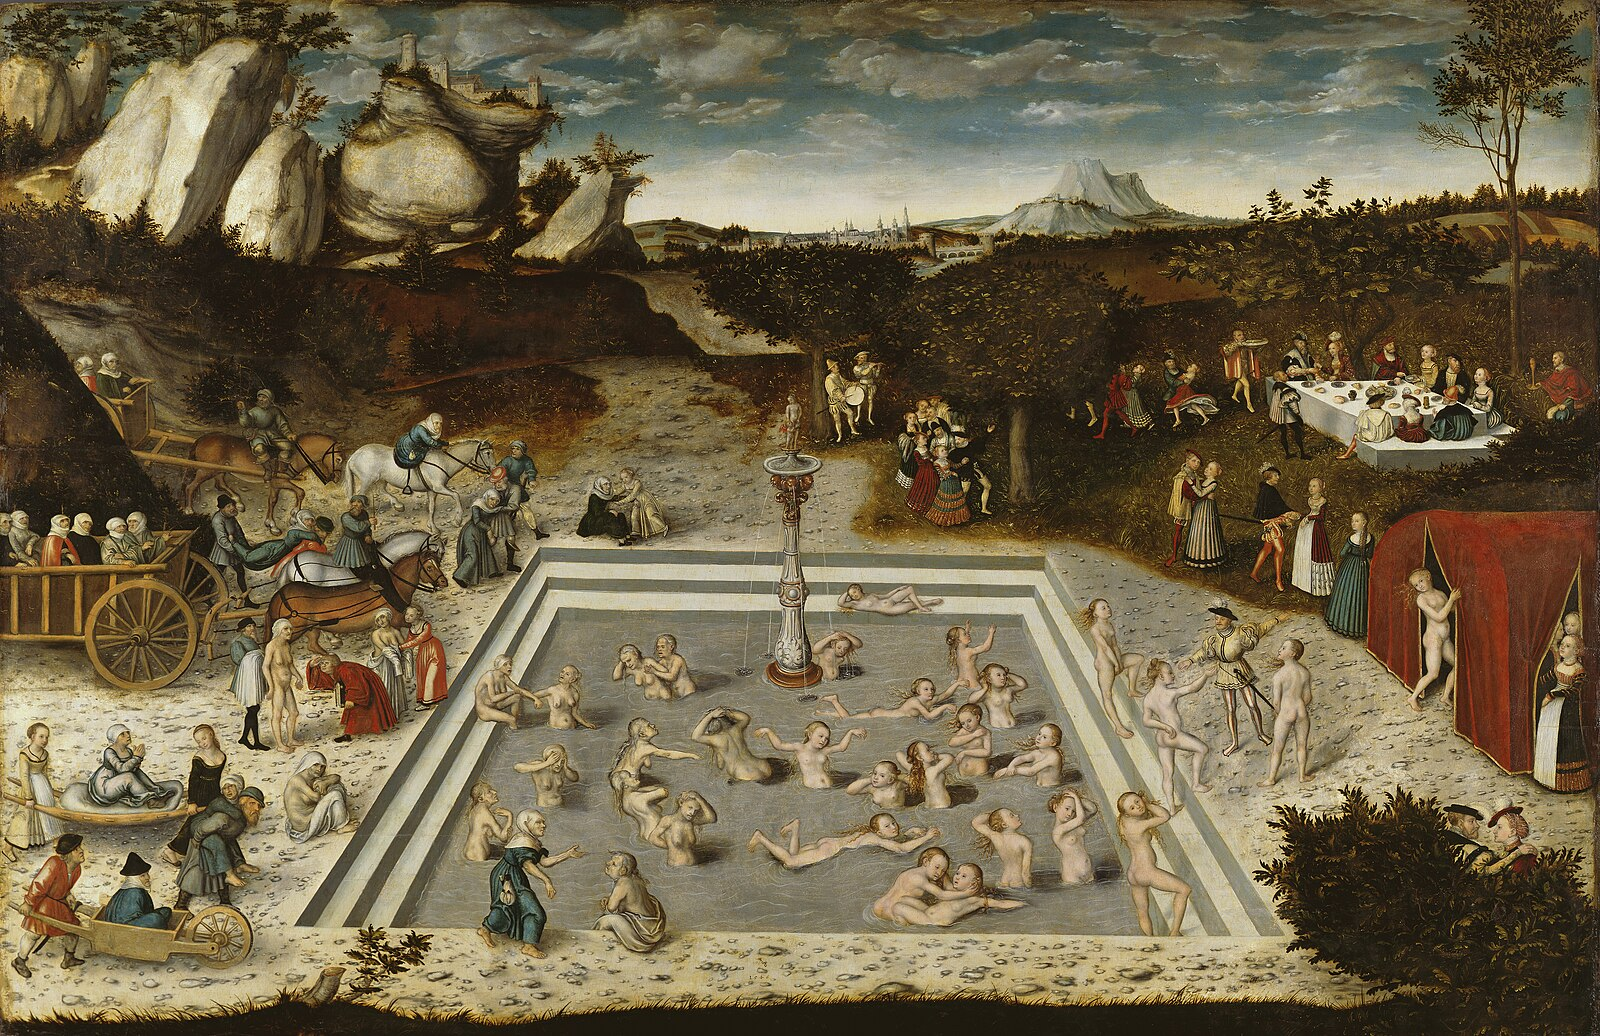
\includegraphics[width=\linewidth]{media/image1.jpg}
    \caption{The Fountain of Youth (1546) by Lucas Cranach the Elder (c. 1472-1553). The oil painting exhibited at the Gemäldegalerie Berlin depicts people's wish to remain youthful forever. License: public domain.}
    \label{fig:fountain}


  \end{fullwidth}

\end{figure}



\begin{figure}[t!]

  \begin{fullwidth}
    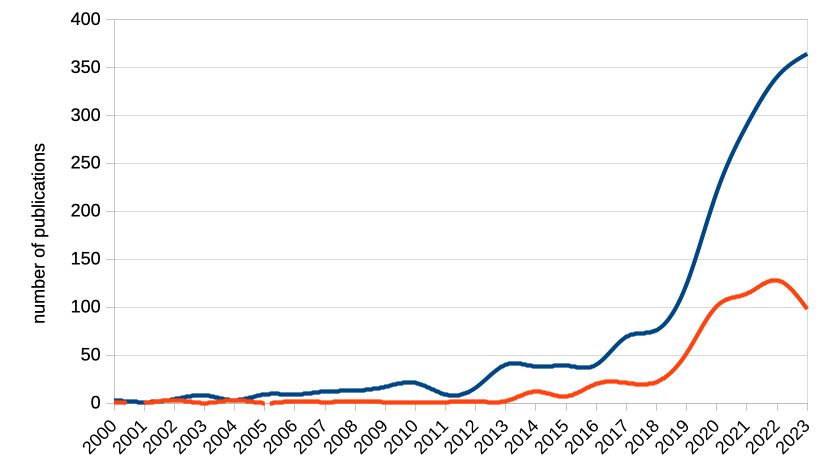
\includegraphics[width=\linewidth]{media/image2.png}
    \caption{Scientific publications on the topics of "intermittent fasting" (blue) and "time-restricted feeding" (red) in the \emph{Web of Science}. The number of publications on the former has increased from less than one per week to more than one per day over the last ten years. From 2014 to 2023, there was almost a tenfold increase. Source: Web of Science (www.webofscience.com), Topic Search}
  \end{fullwidth}
\end{figure}




\section{The study}






The researchers recruited 311 people to take part in the study via calls on social media. The researchers let them choose whether they wanted to stick to the diet (experimental group, TRF, \emph{n }= 231) or not change their eating habits (control group, \emph{n }= 80). Data on cognitive performance, sleep, and subjective well-being were collected at three points in time: shortly before starting the diet, after 1 month, and after 2 months, at the end of the study. In the two groups, 76 of the 231 (33\%) and 29 of the 80 (36\%) participants, respectively, remained. These people were on average 26 years old (range: 18 to 61) and had a slightly higher average body weight in the experimental group (70.6 vs. 65.8 kg) and a slightly higher body mass index (BMI: 24.1 vs. 22.6).







Cognitive tests were used to measure the subjects' attention and cognitive control. Memory span and working memory performance were also assessed. A questionnaire on sleep provided information on, among other things, the duration, interruption, and subjectively experienced quality of sleep. With regard to subjective well-being, the participants were asked to assess the extent to which predefined adjectives (e.g. about anxiety, energy, and happiness) applied to them. Although the results showed a statistically significant effect for the repetition of the various tests on cognitive performance, there was no significant difference between the groups. According to the researchers, the performance improved as a result of repeating the tests, thus a learning effect. Statistically, subjective well-being also improved significantly over time, but again there was no group effect. The authors suggest that this could be due to the fact that the weather improved over the course of the experiment (May to July 2021) and participants were on vacation. There was only a significant group difference in body weight: The BMI of the experimental group actually fell to an average of 23.3, bringing it closer to the value of the control group.







As a result, this study provides no evidence that intermittent fasting in the form of TRF increases cognitive performance or emotional well-being. The study authors already discuss some of the limitations of their study, in particular the lack of randomization. The reason for this was to increase the intrinsic motivation of the participants for the diet. Since two-thirds of the participants in the experimental group stopped within the 2 months of the trial, it is reasonable to assume that the remaining 33\% (\emph{n} = 76) were highly motivated, as there was no financial or other compensation for completing the experiment. In view of this fact, one might have expected at least a placebo or situation effect: Those who are more motivated perhaps exert themselves more in cognitive tests or at least answer the questions about subjective well-being more positively. However, the high motivation could of course have already been present at the first measurement, which would mean that it would no longer be visible in the comparison with the final result.







My biggest objection, though, concerns the short duration of the experimental intervention of only two months. The researchers cite two previous studies for their approach, which reported a positive effect of intermittent fasting on cognitive performance (Leclerc et al., 2020; Ooi et al., 2020). In these studies, however, the intervention lasted 24 and 36 months respectively, i.e. 12 to 18 times as long. In addition to that, Ooi and colleagues had examined a group of older people with symptoms of mild cognitive impairment (Ooi et al., 2020), while the participants in the new study were on average only 26 years old. Since possible changes in cognitive performance or subjective well-being must act via the brain, this raises the complex question of the extent to which a short diet of only two months can effectively improve brain activity. Additionally, the subjects in the experimental group were allowed a transitional phase of one week in which they were only supposed to fast for 14 hours (instead of the 16 hours that should ultimately be achieved) and were even encouraged to interrupt the diet one day a week and eat \emph{ad }\emph{libitem}. This further reduced the actual duration of the comparatively short intervention although it may have prevented even more dropouts.







A general question that I will address in more detail in the next section is that of the ecological validity of such tests. The neuropsychological tests frequently used in this type of research -- as in Leclerc and colleagues (2020) -- were originally developed to measure cognitive impairment in patients with psychological-psychiatric disorders and neurological diseases. It is still unclear what differences in these computer tests mean for the participants' everyday lives, which I described as a possible clinical and normative fallacy in earlier research (Schleim, 2014). The measured differences are also relative, even in the promising study by Leclerc and colleagues: The main statistically significant cognitive finding was that people in the experimental group made 23\% fewer errors in a test of spatial working memory after 12 months and 32\% fewer errors after 24 months; in the control group, they made 23\% fewer errors after 12 months and 16\% fewer errors after 24 months (Leclerc et al., 2020). That is a difference between the groups of 0\% after 12 months and 16\% after 24 months. Note that despite the randomization in this study, there was already a statistically significant different error rate between the two groups at the beginning of the dietary intervention (i.e., 18.9 vs. 24.6 points, \emph{p }< .05), which casts doubt on the groups' cognitive homogeneity (Leclerc et al., 2020). This shows that these results are not only subject to fluctuations but must also be interpreted carefully.







The authors of the new study discuss the interesting idea that the diet could improve psychological functioning by improving sleep quality. This would also provide an answer to the aforementioned question of how brain function can be changed in the short term by fasting. Accordingly, a follow-up study with people with sleep disorders should be considered. However, the difficulties in their present study also reflect the complexity and heterogeneity of real life: People who would like to diet to improve their health and cognition will also be more or less motivated, undergo different seasons, go on vacation, and the like. This illustrates how both controlled experimentation and interventions in one's personal life can consist in trial and error -- and yield ambiguous results. Even rigorous randomized controlled trials often cannot account for all possible confounds and need to simplify their boundary conditions, like the exclusion of patients with comorbidity in psychiatric research, while the patients in clinics often come with more than one mental problem (Hengartner, 2022).







\section{\textbf{Cognitive enhancement}}







Since 2000, an academic discourse has gained importance that deals with the improvement of cognitive performance (less frequently: mood, emotions) in healthy individuals. At first, this was referred to as "cognitive enhancement"; later, the term "neuroenhancement" was also used more commonly (Greely et al., 2008; Schleim \& Quednow, 2018; Schleim, 2023). Following the "Decade of the Brain" (the 1990s), more thought was given to how people outside of therapeutic contexts could also benefit from neuroscience and neurotechnology. Probably due to the increasing use of psychopharmacological drugs, especially stimulants (such as methylphenidate/Ritalin or amphetamine), in the same period, such substances took a central role in the debate, even though methods of electrical or magnetic brain stimulation were discussed as well. Conventional or everyday activities such as physical exercise, sleep, and nutrition have also been discussed as ways of improving cognitive performance (Dresler et al., 2019). In this respect, the new study in the \emph{Journal of Trial and Error, }too, can be classified in this area.







As I mentioned in the previous section, a diet would need to improve brain activity in order to improve mental function. The prefix "psycho" in "psychopharmacological drugs" indicates that these substances act directly on the nervous system. In this respect, psychoactive substances would be a more obvious attempt to influence cognitive performance and subjective well-being. However, this has proven to be much more difficult -- in healthy and well-rested individuals -- than was thought at the beginning of the neuroenhancement debate in the early 2000s (Schleim \& Quednow, 2018; Schleim, 2023). For example, Roberts and colleagues (2020, pp. 20-21) conclude about the stimulants often prescribed for the treatment of attention disorders, when used by people without the diagnosis:






\begin{quote}

  Methylphenidate has the strongest effects on cognition of the three stimulants observed. However, the positive effects are small to moderate, and limited to recall, inhibitory control and sustained attention. [...] D-amphetamine produces no improvements in cognition, and so can probably be ruled out of future investigation for safe, effective cognitive enhancement. The data with these stimulants is far from positive if we consider that effects are small and likely transient, in experiments that do not accurately reflect their actual use in the wider population.

\end{quote}






Even if this does not provide conclusive evidence, it relativizes the expectations of neuroenhancement -- and indirectly also the cognitive improvement through diet: If the scientific results are sobering even with the substances that influence neurotransmitters like dopamine and noradrenaline in the brain, then improvement through food intake is likely to be even more difficult. Here Roberts and colleagues (2020), like me, point out the problem of ecological validity. A few more points or a couple of fewer errors in a neuropsychological test do not necessarily mean a more successful life (Schleim, 2014). In addition to the issue of ecological validity, the lack of long-term studies has also been pointed out for many years, which limits the scientific validity of many studies (Turner \& Sahakian, 2006). This point also played a role in the discussion of the new study on intermittent fasting.







One of the rare exceptions among the already few studies with healthy test subjects asked experienced chess players to alternately play against a chess computer under the influence of placebo, caffeine, methylphenidate or modafinil in a double-blind study design (Franke et al., 2017). The increase in performance (games won) after taking the psychoactive substances was descriptively minimal and not statistically significant for all conditions. However, the study also had low power due to the small number of participants (\emph{n }= 39, all men). In a very competitive competition, though, where the performance of the competitors is close to each other, even small differences can make the difference between winning and losing. In this respect, it is interesting that the performance of the chess players was almost identical for caffeine and methylphenidate (both 4\% more points than for placebo) and was even 2\% higher under the influence of modafinil, a substance used to treat sleep disorders (Franke et al., 2017).







Therefore, in my opinion, such results show that we should avoid exaggerated expectations in research and discussion on the improvement of human beings. Studies on science communication, especially on genetic engineering, have shown many years ago that scientists are under pressure to promise the applicability of their research ("translational pressure") and that scientists as well as their research institutes have an interest in getting media attention (Caulfield \& Condit, 2012). I will discuss a current example in the field of diet research in the last section.







\section{Outlook: Hype, alarmism and reality}







As already mentioned and shown above (Figure 2), the topics of fasting and interval fasting in particular have received a great deal of attention in recent years, both in the scientific community and in the general media. It is not currently foreseeable that this trend will change soon. While this commentary was being written, an interesting example occurred in the media that I would like to briefly discuss here. We could say that after the previous hype on intermittent fasting, we now meet an example of fasting-related alarmism. In any case, it illustrates the translational pressure to make it into the media.







On March 18, 2024, NBC News reported "Intermittent fasting linked to higher risk of cardiovascular death, research suggests" (Bendix, 2024), the \emph{Washington Post} "The intermittent fasting trend may pose risks to your heart" (O'Connor, 2024) and a day later the Dutch NOS "American Heart Association warns against fasting, risk of premature death" (NOS Nieuws, 2024). The fact behind these far-reaching headlines is a poster by Chinese researchers at this year's American Heart Association Epidemiology and Prevention -- Lifestyle and Cardiometabolic Health conference. These scientists are analyzing health data on behalf of the American Heart Association. On March 18, 2024, the Association published a press release about the poster entitled "8-hour time-restricted eating linked to a 91\% higher risk of cardiovascular death", which attracted rapid media attention around the globe (American Heart Association, 2024). The results are preliminary and not yet peer-reviewed. The Dutch headline that the Heart Association itself warns against fasting can probably be regarded as a false report. Notably, the Association added the following caveat a day later: "As noted in all American Heart Association scientific meetings news releases, research abstracts are considered preliminary until published in a peer-reviewed scientific journal." A closer look at the poster in question shows that in the corresponding study on cardiovascular mortality, 423 of 11,831 people who ate for 12 to 16 hours a day, i.e. who did not follow a diet, died during the observation period, compared to 31 out of 414 people who ate for less than 8 hours a day, i.e. who applied intermittent fasting or TRF. From this, the researchers calculated a hazard ratio of 1.9, with a 95\% confidence interval of 1.20 to 3.03. The 91\% increased risk, which the press release and many media reports picked up on, is derived from this.







It would of course be dramatic if people improved their psychological functioning through a diet, but then died earlier because of a disease. However, as the study has not even been published yet, this news should be taken with at least a grain of salt. The whole issue becomes more complex when you consider that intermittent fasting is recommended to reduce obesity, which in turn is associated with cardiovascular disease itself (De Cabo \& Mattson, 2019). This brings us to the contradictory scientific findings that fasting is associated with both more and less cardiovascular (and other) disease. However, as with all observational studies, the data presented on the above poster cannot be used to draw any firm causal inferences. The deaths of the 31 people could have been caused by factors that were not investigated in the study. In the discussion, however, muscle atrophy is brought into play as a possible mechanism for these deaths. Perhaps at least some of these people, who ate for less than 8 hours a day for many years, were simply undernourished?







The new study addresses a topic that is likely to remain relevant for the time to come. Intermittent fasting remains topical, as does the desire for an increase in cognitive performance and mood. To what extent nutrition plays a role not only in reducing or preventing symptoms of illness, but also in improving healthy living, has to be clarified by further research. It is already common wisdom that sufficient physical exercise, good sleep, and a balanced diet are also important for psychological well-being (Dresler et al., 2019; Schleim, 2023; Walsh, 2011). As an alternative to the term "neuroenhancement", I have proposed the term "instrumental substance use" to describe the use of psychoactive substances to improve life more generally (Schleim, 2020). Similarly, one could also speak of "instrumental fasting". However, there still seems to be a long way to go before concrete recommendations for everyday life can be derived from scientific studies.



















\section{References}



\hspace*{\parindent}American Heart Association. (2024, March 18). \emph{8-hour time-restricted eating linked to a 91\% higher risk of cardiovascular death}. Newsroom. \href{https://newsroom.heart.org/news/8-hour-time-restricted-eating-linked-to-a-91-higher-risk-of-cardiovascular-death/}{https://newsroom.heart.org/news/8-hour-time-restricted-eating-linked-to-a-91-higher-risk-of-cardiovascular-death/}







Bendix, A. (2024, March 18). \emph{Intermittent fasting linked to higher risk of cardiovascular death, research suggests}. NBC News\emph{.} \url{https://www.nbcnews.com/health/heart-health/intermittent-fasting-risk-cardiovascular-death-rcna143853}







Caulfield, T., \& Condit, C. (2012). Science and the sources of hype. \emph{Public Health Genomics}, \emph{15}(3-4), 209-217. \url{https://doi.org/10.1159/000336533}







Center for Healthy Aging (n.d.). \emph{Center for Healthy Aging. }University of Copenhagen. \url{https://healthyaging.ku.dk}







De Cabo, R., \& Mattson, M. P. (2019). Effects of intermittent fasting on health, aging, and disease. \emph{New England Journal of Medicine}, \emph{381}(26), 2541-2551. \url{https://doi.org/10.1056/NEJMra1905136}







Dresler, M., Sandberg, A., Bublitz, C., Ohla, K., Trenado, C., Mroczko-Wasowicz, A., Kühn, S., \& Repantis, D. (2019). Hacking the brain: dimensions of cognitive enhancement. \emph{ACS Chemical Neuroscience}, \emph{10}(3), 1137-1148. \url{https://doi.org/10.1021/acschemneuro.8b00571}







Franke, A. G., Gränsmark, P., Agricola, A., Schühle, K., Rommel, T., Sebastian, A., Balló, H. E., Gorbulev, S., Gerdes, C., Frank, B., Ruckes, C., Tüscher, O., \& Lieb, K. (2017). Methylphenidate, modafinil, and caffeine for cognitive enhancement in chess: A double-blind, randomised controlled trial. \emph{European Neuropsychopharmacology}, \emph{27}(3), 248-260. \url{https://doi.org/10.1016/j.euroneuro.2017.01.006}







Greely, H., Sahakian, B., Harris, J., Kessler, R. C., Gazzaniga, M., Campbell, P., \& Farah, M. J. (2008). Towards responsible use of cognitive-enhancing drugs by the healthy. \emph{Nature}, \emph{456}(7223), 702-705. \url{https://doi.org/10.1038/456702a}







Hengartner, M. P. (2022). \emph{Evidence-biased Antidepressant Prescription: }\emph{Overmedicalisation}\emph{, Flawed Research, and Conflicts of Interest}. Palgrave Macmillan. \url{https://doi.org/10.1007/978-3-030-82587-4}







Johnstone, A. (2015). Fasting for weight loss: An effective strategy or latest dieting trend? \emph{International Journal of Obesity}, \emph{39}(5), 727-733. \url{https://doi.org/10.1038/ijo.2014.214}







Leclerc, E., Trevizol, A. P., Grigolon, R. B., Subramaniapillai, M., McIntyre, R. S., Brietzke, E., \& Mansur, R. B. (2020). The effect of caloric restriction on working memory in healthy non-obese adults. \emph{CNS Spectrums}, \emph{25}(1), 2-8. \url{https://doi.org/10.1017/S1092852918001566}







Leiden University (n.d.). \emph{Healthy Ageing.} Leiden University. \url{https://www.universiteitleiden.nl/en/research-dossiers/taking-care-of-your-health/healthy-ageing}







NOS Nieuws (2024, March 19). \emph{Amerikaanse hartstichting waarschuwt voor vasten, kans op voortijdig overlijden.} NOS. \href{https://nos.nl/artikel/2513387-amerikaanse-hartstichting-waarschuwt-voor-vasten-kans-op-voortijdig-overlijden}{https://nos.nl/artikel/2513387-amerikaanse-hartstichting-waarschuwt-voor-vasten-kans-op-voortijdig-overlijden}







O'Connor, A. (2024, March 18). The intermittent fasting trend may pose risks to your heart. \emph{The Washington Post.} \url{https://www.washingtonpost.com/wellness/2024/03/18/intermittent-fasting-time-restricted-eating/}







Ooi, T. C., Meramat, A., Rajab, N. F., Shahar, S., Ismail, I. S., Azam, A. A., \& Sharif, R. (2020). Intermittent fasting enhanced the cognitive function in older adults with mild cognitive impairment by inducing biochemical and metabolic changes: A 3-year progressive study. \emph{Nutrients}, \emph{12}(9), Article 2644. \url{https://doi.org/10.3390/nu12092644}







Roberts, C. A., Jones, A., Sumnall, H., Gage, S. H., \& Montgomery, C. (2020). How effective are pharmaceuticals for cognitive enhancement in healthy adults? A series of meta-analyses of cognitive performance during acute administration of modafinil, methylphenidate and D-amphetamine. \emph{European Neuropsychopharmacology}, \emph{38}, 40-62. \url{https://doi.org/10.1016/j.euroneuro.2020.07.002}







Schleim, S. (2014). Whose well-being? Common conceptions and misconceptions in the enhancement debate. \emph{Frontiers in Systems Neuroscience}, 8, Article 148. \url{https://doi.org/10.3389/fnsys.2014.00148}







Schleim, S. (2020). Neuroenhancement as instrumental drug use: Putting the debate in a different frame. \emph{Frontiers in Psychiatry}, \emph{11}, Article 567497. \url{https://doi.org/10.3389/fpsyt.2020.567497}







Schleim, S. (2023). \emph{Mental Health and Enhancement: Substance Use and Its Social Implications}. Palgrave Macmillan. \url{https://doi.org/10.1007/978-3-031-32618-9}







Schleim, S., \& Quednow, B. B. (2018). How realistic are the scientific assumptions of the neuroenhancement debate? Assessing the pharmacological optimism and neuroenhancement prevalence hypotheses. \emph{Frontiers in Pharmacology}, \emph{9}, Article 315603. \url{https://doi.org/10.3389/fphar.2018.00003}







Turner, D. C., \& Sahakian, B. J. (2006). Neuroethics of Cognitive Enhancement. \emph{BioSocieties}, \emph{1}(1), 113-123.







University Medical Center Groningen (n.d.). \emph{Healthy Ageing. }UMCG Research. \url{https://umcgresearch.org/w/healthy-ageing}







Walsh, R. (2011). Lifestyle and mental health. \emph{American }\emph{Psychologist}, \emph{66}(7), 579-592. \url{https://doi.org/10.1037/a0021769}


\end{document}